% Define the chapter heading image to be used for all (subsequent) chapters.
%\chapterimage{ChapterImage.jpg} % Chapter heading image

%\chapter{Dedication}\label{dedication}

This book is dedicated to my wife Alison, who has tolerated my need to ``play'' with computers for many, many years. She doesn't understand how or why I can work with computers all day, then come home and still want to play with them in my free time. It's a woman thing - they just don't understand :o)

She thinks that I \emph{need to get a life} - which I think means
\emph{go shopping}!

Dedicated also to all those \emph{Open Source} people out there, who spend time and effort creating wonderful pieces of software and hardware, and then they make them all available for free. You know who you are.

%\section*{Introduction}\label{introduction}

This book is for those of us who have played with, and perhaps mastered,
the Arduino in its various forms, and who need now to move up to
programming it - or home made clones on breadboards or stripboard (or
even, home made PCBs) and so on - in plain vanilla C code.

This need could be for many reasons, running out of space, too slow,
lots of hidden things going on that are interfering with the project we
have in mind etc. You might even have found that you can replace a full
Arduino with a small AtTiny85, for example, and get exactly the same
results, for a lot less outlay.

This book should help with that migration. It's not difficult, but it's
not easy either. You will have to think a lot more at the hardware
level, which the Arduino environment abstracts away for you, to make it
simple.

Interrupts, timers and sleep modes will figure largely in what we do
with AVR programming - we don't want to be wasting time waiting for
someone to press a switch, or a sensor to register a reading, for
example. And if there's nothing for the AVR to do while it waits around,
we let it sleep! This saves power and could mean the difference between
your project being able to run for months, if not years, on a couple of
batteries, and having to be constantly plugged into the mains.

Just remember, \texttt{delay()} is not your best friend when programming
the Arduino or the AVR. Hopefully, you will find this out later when you
read on.

\subsection*{Hardware Necessary}\label{hardware-necessary}

\begin{itemize}
\item
  An Arduino, perhaps. It's not essential, but you can use one to
  program bare AVR microcontrollers if you don't have a ISP programmer.
  A \emph{Nano} or \emph{Uno} etc are probably best. The Mega is perhaps
  a tad overkill as an ISP programmer!
\item
  If you don't have a spare Arduino lying around, then you will need an
  ISP programmer. I got mine on eBay for around £3.28 including postage,
  from a seller named finetech007, in China. Other suppliers are
  available. The programmer allows you to save the 2Kb that an Arduino
  bootloader takes up, but obviously stops you programming the device
  using that bootloader.

  Don't worry if you don't have an ISP programmer, as mentioned above,
  your existing Arduino can be used to program (other) AVR
  micro-controllers. And if you don't have an Arduino, why not build
  your own? Grab hold of a
  \href{http://start.shrimping.it/project/protected/build.html}{Protected
  Shrimp} kit for around £10.00\footnote{Prices correct at the time of
    writing.}, or a more permanent (some soldering required)
  \href{http://start.shrimping.it/kit/stripboard.html}{Copper Shrimp}
  add on kit for £1.90 from those nice people at
  \href{http://start.shrimping.it//index.html}{ShrimpingIT}. I started
  with an Arduino Duemilanove which was bought for me as a gift, but I
  built my own Shrimp Kit just for the fun of it. I've built a few more
  since then!
\item
  A breadboard and assorted components, wires, etc. This is limited to
  the odd switch, LED and such like. Maybe a shift register or two will
  be handy - it depends on what you are expecting to achieve with the
  AVR. (Or, what I decide to include in the book!)
\end{itemize}

\section*{Image Credits}\label{image-credits}

The front cover image on this book is taken from the book \emph{Kunstformen der Natur}
by German biologist Ernst Haeckel. The book was published between 1899 and 1904. The
image used is of various \emph{Polycystines} which are a specific kind of micro-fossil.

You can read about them at \url{https://en.wikipedia.org/wiki/Polycystine} and there is a
brief overview of the above book at \url{https://en.wikipedia.org/wiki/Kunstformen_der_Natur}
which shows a number of other images.

Polycystines have absolutely nothing to do with the Arduino or AVR microcontrollers,
but I liked the image, and because it is in the Public Domain, I decided that it would
make a good cover image

\subsection*{Coming Up}\label{coming-up}


% The main meat of the book begins here.
%\mainmatter

\part{PlatformIO}\label{part-platformio}
\chapter{Installing PlatformIO}\label{installing-platformio}

\section{PlatformIO}\label{platformio}\index{PlatformIO}

\href{http://platformio.org/}{PlatformIO} is a command line\footnote{Panic
  not Windows users, the command line is not your mortal enemy. In fact,
  you can get stuff done a lot quicker in the command line, \emph{most}
  of the time. Once you get to know it of course.} and IDE based utility
that allows you to write plain C or C++ code to upload to your Arduino,
or, almost any other embedded microcontroller that is known to man,
woman or hamster! At the time of writing, 5th July 2017, PlatformIO
supported:

\begin{itemize}
\tightlist
\item
  23 Development Platforms
\item
  13 Frameworks
\item
  412 Embedded Boards
\item
  61 Project Examples
\item
  1,738 Libraries
\item
  8,084 Library Examples
\end{itemize}

You can use it to replace the Arduino IDE too, if you wish, as it
understands plain Arduino code as well as AVR C code. Arduino sketches
can be imported unchanged, worked on, compiled and uploaded without any
difficulty.

PlatformIO comes in two main flavours:

\begin{itemize}
\tightlist
\item
  The command line version\footnote{See previous footnote!}
\item
  An IDE version for the Atom editor, or Visual Studio. This also allows
  you to run the command line commands without having to install that
  package separately.
\end{itemize}

In addition, there's a lot of documentation on the web site about how
you can install the PlatformIO tools into a large number of different
IDEs, some of which you may already be using.

\subsection{Installing Atom}\label{installing-atom}

As a lot of Windows people \emph{might} not be fully acquainted with the command
line, I've decided to base the remainder of this book on using the Atom editor
from Github, and the PlatformIO package for it. 

\textbf{To Be COMPLETED}

\subsection{Installing PlatformIO in
Atom}\label{installing-platformio-in-atom}

We will install the following 2 PlatformIO packages for Atom:

\begin{itemize}
\tightlist
\item
  platformio-ide (version 2.0.0 beta 7 is the latest at the time of
  writing)
\item
  platformio-ide-debugger (version 1.2.3 is the latest at the time of
  writing)
\end{itemize}

Open Atom and select the \lstinline!edit -> Preferences! menu option.
When the `Settings' tab appears, look down to find the option labelled
`+ Install' and choose it.

Search for `platformio' and a list of available options will soon be
displayed. Find the two packages mentioned above and click the `install'
button. Wait \ldots{}.

Eventually you will be prompted to restart Atom, so do so.

If, on the restart, you are prompted to Install Clang go ahead and do
so, if you wish, or select \lstinline!Disable Code Completion!. Clang
will have to be installed using your package manager - it's not a
package for Atom but for the entire system. Full details are
\href{http://docs.platformio.org/en/latest/ide/atom.html\#ii-clang-for-intelligent-code-completion}{here}.

Full instructions on installing Atom and PlatformIO packages can be
found
\href{http://docs.platformio.org/en/latest/ide/atom.html\#clang-for-intelligent-code-completion}{here}.

You will know that you have installed PlatformIO when you restart Atom
and see a `bug face' looking back at you from the PlatformIO welcome
screen.

\section{PlatformIO Quick Start}\label{platformio-quick-start}

\subsection{Create the Blink Project}\label{create-the-blink-project}

Open the Atom editor, if not already running, and make sure that you can
see the PlatformIO Welcome Screen. Click on `+ New Project' to start the
New Project Wizard.

You must first select a board. As I'm using an Arduino Nano, for this
example, that's what I'll be selecting. You may choose something
different.

You will hopefully notice that when you have selected a board, you get
to select another, and another \ldots{}. this is a feature of PlatformIO
in that it allows you to use the same source code for multiple boards
and/or microcontrollers. Nice. I sometimes build for the Nano, the Uno,
the Duemilenova and for the stand-alone AtTiny85.

For now, however, let's stick with a single board.

Now select a directory to save the code in. My choice is:

\begin{quote}
\lstinline!/home/norman/SourceCode/PlatformIO/Blink!
\end{quote}

you might want to choose something different, especially if you are on
Windows!

Click the `Process' button.

The first time PlatformIO is used, it needs to connect to the internet
to install the appropriate tools for the board you have chosen. In the
case of the Nano, this is `platform: atmelavr'. Just wait \ldots{}.

When the processing has completed, the output directory that you chose
above will be populated by a number of files and directories:

\begin{itemize}
\tightlist
\item
  A directory named \lstinline!lib! and a file, \lstinline!readme.txt! within.
  The readme file has all the information you will need if you intend to
  write some libraries for this particular project. The source code for
  the libraries should be kept in this directory.
\item
  A directory named \lstinline!src!. This is where you will create your own
  project's source code.
\item
  A file named \lstinline!.gitignore!. This (hidden on Linux) file tells git, if in use for
  version control, to ignore a number of files that are not required in
  normal circumstances, usually files that can be recreated at will.
\item
  A file named \lstinline!.travis.yml!. This (hidden on Linux) file is a YAML source file that
  tells the Travis `Continuous Integration' system what to do whenever
  something in the project changes. We will not be using this feature.
\item
  A file named \lstinline!platformio.ini!. This file tells PlatformIO how the
  project will be built and uploaded to the microcontroller, for each
  board you selected when creating the project.
\end{itemize}

\subsection{Write the Blink Code}\label{write-the-blink-code}

Now we have our project (Blink) created, we need to write some code, so:

\begin{itemize}
\tightlist
\item
  Right-click the `src' folder in the `Project' tab, and select
  \lstinline!New File! from the context menu that appears.
\item
  Enter the file name when prompted, I chose `blink.c', but you can name
  the file as you wish.
\end{itemize}

The new file opens in the editor, so add the following code:

\begin{lstlisting}[language=C,caption={AVRBlink.c}]
// Define the CPU speed, if not already defined.
// My Nano is running at 16 MHz, so 16 million it shall be.
// This allows the CPU to correctly set Baud rates, delays etc.
//
// This must also be done before anything else.
#define F_CPU 16000000UL // 16 MHz clock speed

// Pull in the header files for the AVR and the delay utilities. the
// avr/io header will correctly pull in the appropriate other header 
// file for our chosen CPU. Neat!
#include <avr/io.h>
#include <util/delay.h>

// The main code starts here. Always. Although main() appears to return
// an int value, it never will because microcontrollers never exit 
// from main(). The compiler might complain about it though, but it's 
// only a warning.
int main(void)
{
  // SETUP goes here.
  //Makes D13 aka PB5 (PORTB, Pin5) an Output
  DDRB = (1 << PB5); 

  // And here is what Arduino calls loop.
  while(1) //infinite loop
  {
    // Turn on D13 LED.
    PORTB =  (1 << PB5);
    _delay_ms(1000);

    // Turn off D13 LED.
    PORTB= 0x00; //Turns OFF All LEDs
    _delay_ms(1000); //1 second delay
  }
}
\end{lstlisting}

\subsection{Compile the Code}\label{compile-the-code}

Save the file, \lstinline!File -> Save! or Ctrl-S, then select
\lstinline!PlatformIO -> Build! or Ctrl-Alt-B to build the program. The
compiler messages will appear, and then vanish after a couple of
seconds. Click \lstinline!PlatformIO -> Toggle Build Panel! or press F8
to display them again.

\subsection{Check for Build Errors}\label{check-for-build-errors}

You will see something like the following:

\begin{lstlisting}
Processing nanoatmega328 ...
------------------------------
Verbose mode can be enabled via `-v, --verbose` option
Collected 27 compatible libraries
Looking for dependencies...
Project does not have dependencies
Compiling .pioenvs/nanoatmega328/src/blink.o

src/blink.c:6:0: warning: "F_CPU" redefined

#define F_CPU 16000000UL // 16 MHz clock speed
^
<command-line>:0:0: note: this is the location of the previous 
definition

Linking .pioenvs/nanoatmega328/firmware.elf
Building .pioenvs/nanoatmega328/firmware.hex
Calculating size .pioenvs/nanoatmega328/firmware.elf
AVR Memory Usage
----------------
Device: atmega328p

Program:     178 bytes (0.5% Full)
(.text + .data + .bootloader)

Data:          0 bytes (0.0% Full)
(.data + .bss + .noinit)
========================= [SUCCESS] Took 0.90 seconds ===============
\end{lstlisting}

It appears we have a slight problem, we have redefined F\_CPU.
PlatformIO knows that an Arduino Nano with an AtMega328 runs with a 16
MHz crystal, so it defines the correct speed for us. This is defined in the file
\lstinline!/home/norman/.platformio/packages/framework-arduinoavr/boards.txt! (well, it
is for me anyway, your mileage may vary.) where a number of other details are defined
to make the system aware of the device, the speeds, baud rates for uploads etc.

We can either:

\begin{itemize}
\item
  delete the offending line of code in our \lstinline!blink.c! file, or;
\item
  Wrap the code in sentinels, and only define it if it isn't already
  define. To do this amend line 6 to the following:

\begin{lstlisting}[language=C,firstnumber=6,caption={Fixing F\_CPU warning in AVRBlick.c}]
#ifndef F_CPU
#define F_CPU 16000000UL // 16 MHz clock speed
#endif
\end{lstlisting}
\end{itemize}

Then recompile. The warning should now go away. You might need to press
F8 again to view the compiler output.

\subsection{Gosh, Look How Small it
is!}\label{gosh-look-how-small-it-is}

Look at the last few lines of the compiler output text:

\begin{lstlisting}[firstnumber=19]
AVR Memory Usage
----------------
Device: atmega328p

Program:     178 bytes (0.5% Full)
(.text + .data + .bootloader)

Data:          0 bytes (0.0% Full)
(.data + .bss + .noinit)
\end{lstlisting}

This is telling you that the entire blink program takes up \emph{only}
178 bytes of Flash Memory and zero bytes of data space (in the Dynamic
RAM), on the Nano. What does it take up on an Arduino? Lets see:

\begin{lstlisting}
Sketch uses 928 bytes (3%) of program storage space. ....

Global variables use 9 bytes (0%) of dynamic memory, ....
\end{lstlisting}

We have a huge saving in such a tiny program. Just out of interest, I
compiled the BareMinimum Arduino example, which looks like this:

\begin{lstlisting}[language=C]
void setup() {
  // put your setup code here, to run once:
}

void loop() {
  // put your main code here, to run repeatedly:
}
\end{lstlisting}

And the compiler told me that:

\begin{lstlisting}
Sketch uses 444 bytes (1%) of program storage space. ....

Global variables use 9 bytes (0%) of dynamic memory, ....
\end{lstlisting}

So, our blink code, written in AVR C with none of the Arduino wrappings,
takes up only 40\% of the space used in Flash Memory by a completely
empty\footnote{More on the reasons why elsewhere.} Arduino sketch!

\subsection{Upload to Our Board}\label{upload-to-our-board}

Now that we have a clean build, we can upload it to our device. The
first time we do this with an AVR device, Arduino etc, we will need to
download the \lstinline!avrdude! tool. This is what we need to program
our device.

Select \lstinline!PlatformIO -> upload! and wait\ldots{}

Press F8 if the build information vanishes again.

You might see the following, on Linux:

\begin{lstlisting}
Warning! Please install `99-platformio-udev.rules` and check that your 
board's PID and VID are listed in the rules.
https://raw.githubusercontent.com/platformio/platformio/
develop/scripts/99-platformio-udev.rules
\end{lstlisting}

(The filename above is all on one line, I've split it to fit on the page.)

This is required to allow non-root users on a Linux system, the ability
to upload using the USB ports. 

On some systems you might need to add your 
user to the group \lstinline!dialout! or possibly \lstinline!plugdev! and 
restart your Atom session to pick up the new group. You can find the correct group
as follows:

\begin{lstlisting}[language=bash]
grep -i -e dialout -e plugdev /etc/group

dialout:x:18:
\end{lstlisting}

In my case, on Centos 7, it's the \lstinline!dialout! group, so:

\begin{lstlisting}[language=bash]
sudo usermod -a -G dialout $USER
\end{lstlisting}


\subsubsection{Install the Rules File}\label{install-the-rules-file}

Download and install the rules file as follows:

\begin{lstlisting}[language=bash]
cd /tmp

# The following is all on ONE LINE!
sudo wget https://raw.githubusercontent.com/platformio/platformio/
develop/scripts/99-platformio-udev.rules

sudo cp 99-platformio-udev.rules /etc/udev/rules.d/

sudo service udev restart
cd -
\end{lstlisting}

or, if that fails:

\begin{lstlisting}[language=bash]
sudo udevadm control --reload-rules
sudo udevadm trigger
cd -
\end{lstlisting}

\section{Don't Forget Your Port}

\chapter{Using the PlatformIO Command Line}\label{using-the-platformio-command-line}

\section{PIO Introduction}\label{pio-introduction}

Windows users, look away now! Only kidding, it's not that bad, honest. 

If you have your own favourite editor, then there's nothing stopping you from using it to create and edit your AVR code, You should either have downloaded and installed the command line version of \indexasis{PlatformIO Core}, or, installed the \indexasis{PlatformIO IDE} and then chosen the option to install the command line commands into your system, as described in \reference{installing-shell-commands}. 

Once installed, whichever method you choose, there are two new commands available, \inline{platformio} or \inline{pio}. They are both the same, and to save wearing out my keyboard, I shall only be using the latter!

\section{Creating a New Project}\label{creating-a-new-project}

\subsection{Finding Our Micro Controller}\label{finding-our-micro-controller}

To create a new project, we need to know where our code will be stored, and which micro controller(s) we wish to use. If we assume that we are using an \indexasis{Arduino} nano, with an \indexasis{ATmega328P} micro controller, then we can find out what we need to use to indicate this when we create the new project. The command:

\begin{lstlisting}[language={bash},numbers={none},caption={PIO - Listing Supported Boards}]
pio boards
\end{lstlisting}

will list all known boards that are supported. As there are quite a few, we should attempt to reduce the amount of output by filtering through \inline{grep} (Linux users) or \inline{find} if we are on Windows:

\begin{lstlisting}[language={bash},numbers={none},caption={Linux - PIO - Listing Arduino Nano Boards}]
pio boards | grep -i nano 
\end{lstlisting}    

The output from the above will resemble the following. The headings will not be included in the output however, I have added those for clarity.

\begin{lstlisting}[numbers={none},caption={PIO - List of Arduino Nano Boards}]
ID                MCU         Frequency ....
nanoatmega168     ATMEGA168   16Mhz     ....
nanoatmega328     ATMEGA328P  16Mhz     ....
nano32            ESP32       240Mhz    ....
redBearLabBLENano NRF51822    16Mhz     ....
redbear_blenano2  NRF52832    64Mhz     ....
\end{lstlisting}    

A similar output will be displayed on windows with the following command:

\begin{lstlisting}[language={bash},numbers={none},caption={Windows - PIO - Listing Arduino Nano Boards}]
pio boards | find /i "nano" 
\end{lstlisting}    

The first column is the id code that we are interested in when we wish to initialise a new project. As we are looking for an \indexasis{Arduino} Nano with an \indexasis{ATmega328P} micro controller, then the second entry looks most promising - it lists the micro controller (MCU) as an ATMEGA328P running at 16MHz, this is definitely what we are looking for. We should note the board id in the first column.


\subsection{Initialise the New Project}\label{initialise-the-new-project}

We are now ready to initialise a new project for our Nano. We do need to create a new directory for the project, as the initialisation assumes that the project directory exists. Once created we can initialise the new project:

\begin{lstlisting}[language={bash},numbers={none},caption={PIO - Initialising a New Project}]
mkdir Nano328P
pio init --project-dir Nano328P --board nanoatmega328
\end{lstlisting}    
    

The command will output the following when it has completed the initialisation:

\begin{lstlisting}[numbers={none},caption={PIO - New Project Initialisation Complete}]
The next files/directories have been created in /SourceCode/Nano328P
platformio.ini - Project Configuration File
src - Put your source files here
lib - Put here project specific (private) libraries

Project has been successfully initialized!
Useful commands:
`platformio run` Process/build project from the current directory
`platformio run --target upload` Upload firmware to embedded board
`platformio run --target clean` Clean project (remove compiled files)
`platformio run --help` Additional information
`platformio run --target program` Upload firmware with ISP Programmer
\end{lstlisting}    

\begin{note}
Actually, the output from the initialisation \emph{does not} mention that you might like to program the AVR with an \indexasis{ISP Programmer}, rather than the normal \indexasis{Arduino} style USB cable. I have added that as an additional useful command as I use both methods of uploading to my AVRs. (The last line above is the one I added.)
\end{note}

Now we can check the contents of the project directory, to see what has been created:

\begin{lstlisting}[language={bash},numbers={none},caption={PIO - Checking New Project Initialisation}]
ls Nano328P
\end{lstlisting}    
    
\begin{lstlisting}[numbers={none},caption={PIO - Checking New Project Initialisation - Result}]
lib  platformio.ini  src
\end{lstlisting}    


\subsection{Creating the Source Code}\label{creating-the-source-code}

To create the source code, we would change into the newly initialised directory, and start editing with our favourite editor. 

\begin{lstlisting}[language={bash},numbers={none},caption={PIO - Creating New Project Source Files}]
cd Nano328P/src
vi AVRSmallBlink.c
...
\end{lstlisting}    

To compile the code, we need to be back up one level in the project's main directory:

\begin{lstlisting}[language={bash},numbers={none},caption={PIO - Compiling the New Project}]
cd ..
pio run 
\end{lstlisting}    

\begin{lstlisting}[numbers={none},caption={PIO - Compiling the New Project - Output}]
[Wed Sep  6 12:31:46 2017] Processing nanoatmega328 (platform: atmelavr; board: nanoatmega328; framework: arduino)
...
Looking for dependencies...
No dependencies
Compiling .pioenvs/nanoatmega328/src/AVRSmallBlink.o
Archiving .pioenvs/nanoatmega328/libFrameworkArduinoVariant.a
Indexing .pioenvs/nanoatmega328/libFrameworkArduinoVariant.a
Compiling .pioenvs/nanoatmega328/FrameworkArduino/CDC.o
...
Archiving .pioenvs/nanoatmega328/libFrameworkArduino.a
Indexing .pioenvs/nanoatmega328/libFrameworkArduino.a
Linking .pioenvs/nanoatmega328/firmware.elf
Calculating size .pioenvs/nanoatmega328/firmware.elf
AVR Memory Usage
----------------
Device: atmega328p

Program:     158 bytes (0.5% Full)
(.text + .data + .bootloader)

Data:          0 bytes (0.0% Full)
(.data + .bss + .noinit)

Building .pioenvs/nanoatmega328/firmware.hex
\end{lstlisting} 

The first time a project is built, there's a number of files to be compiled in addition to the main source file(s) that we created, so there's quite a lot of output on screen. Subsequent builds don't produce as much output. (Unless you have cleaned things out of course - see below.)


\subsection{Uploading the Firmware}\label{uploading-the-firmware}

To upload the compiled firmware file to the Nano, using the USB cable in the normal manner, proceed as follows:

\begin{lstlisting}[language={bash},numbers={none},caption={PIO - Uploading the Firmware}]
pio run --target upload
\end{lstlisting}    

The output from the above will resemble this:

\begin{lstlisting}[numbers={none},caption={PIO - Uploading the Firmware - Output}]
<<< STUFF TO GO HERE >>>
\end{lstlisting}

Alternatively, if you are using one, the commands to upload the code to the Nano using the \indexasis{ISP Programmer}, is as follows and assumes you have set up the \path{platformio.ini} file as explained in \reference{upload-to-our-board}.

\begin{lstlisting}[language={bash},numbers={none},caption={PIO - Programming the Firmware with the ISP Programmer}]
pio run --target program
\end{lstlisting}    

The output from the above will resemble this:

\begin{lstlisting}[numbers={none},caption={PIO - Programming the Firmware - Output}]
<<< STUFF TO GO HERE >>>
\end{lstlisting}


\subsection{Cleaning up After the Build}\label{cleaning-up-after-the-build}

Cleaning out the workfiles etc left behind by the compiler, and returning your project directory to a pristine conddition, containing only \emph{our} source files, is as simple as:

\begin{lstlisting}[language={bash},numbers={none},caption={PIO - Project Cleaning}]
pio run --target clean
\end{lstlisting}    

The output from the \inline{clean} command will be similar to the following:

\begin{lstlisting}[numbers={none},caption={PIO - Project Cleaning - Results}]
[Wed Sep  6 12:35:55 2017] Processing nanoatmega328 (platform: atmelavr; board: nanoatmega328; framework: arduino)
...
Removed .pioenvs/nanoatmega328/libFrameworkArduinoVariant.a
Removed .pioenvs/nanoatmega328/libFrameworkArduino.a
...
Removed .pioenvs/nanoatmega328/FrameworkArduino/wiring_pulse.o
Removed .pioenvs/nanoatmega328/FrameworkArduino/wiring_shift.o
Done cleaning
\end{lstlisting}    

\section{Getting Help}\label{section-getting-help}

The various commands allowed by the \inline{pio} utility are easily obtained:

\begin{lstlisting}[language={bash},numbers={none},caption={PIO - Getting Help}]
pio --help

Usage: pio [OPTIONS] COMMAND [ARGS]...

Options:
  --version          Show the version and exit.
  -f, --force        Force to accept any confirmation prompts.
  -c, --caller TEXT  Caller ID (service).
  -h, --help         Show this message and exit.

Commands:
  account   Manage PIO Account
  boards    Embedded Board Explorer
  ci        Continuous Integration
  debug     PIO Unified Debugger
  device    Monitor device or list existing
  home      PIO Home
  init      Initialize PlatformIO project or update existing
  lib       Library Manager
  platform  Platform Manager
  remote    PIO Remote
  run       Process project environments
  settings  Manage PlatformIO settings
  test      Local Unit Testing
  update    Update installed platforms, packages and libraries
  upgrade   Upgrade PlatformIO to the latest version
\end{lstlisting}    

And help for the individual commands listed can be obtained as follows:

\begin{lstlisting}[language={bash},numbers={none},caption={PIO - Getting Help on Commands}]
pio <command> --help
\end{lstlisting}    

For example:

\begin{lstlisting}[language={bash},numbers={none},caption={PIO - Getting Help on Commands}]
pio account --help
\end{lstlisting}

Which would result in:

\begin{lstlisting}[numbers={none},caption={PIO - Getting Command Help}]
Usage: pio account [OPTIONS] COMMAND [ARGS]...

Options:
  -h, --help  Show this message and exit.

Commands:
  forgot    Forgot password
  login     Log in to PIO Account
  logout    Log out of PIO Account
  password  Change password
  register  Create new PIO Account
  show      PIO Account information
  token     Get or regenerate Authentication Token
\end{lstlisting}






\part{The Atmel AVR}\label{part-atmel-avr}
\chapter{Atmel AVR}\label{atmel-avr}

\section{Introduction}\label{avr-introduction}

The Atmel AVR is the micro controller at the heart of your \indexasis{Arduino} and comes in many different varieties. We are concentrating, in the main, on the Atmel ATmega328P which is the micro controller on the Duemilanove, the UNO and the Nano - although the Nano uses a surface mount version of the 328.

Some clones may also use the surface mounted version of the 328 - it depends. The \indexasis{Arduino} hardware is open source, so anyone is able to build their own clones, using whatever equivalent micro controllers they can source.

\section{Data Sheets}\label{data-sheets}\index{Data Sheets}

You should, if you have not already done so, download the full data sheet for the ATmega320P from \href{http://www.atmel.com/Images/Atmel-42735-8-bit-AVR-Microcontroller-ATmega328-328P_Datasheet.pdf}{Atmel's web site} - don't worry about the fact that the document is over 440 pages long, we \emph{won't} be reading it from start to finish!

Normally, it's good to get an overview of the micro controller, especially when it's new to us, by reading  through the first few chapters which describe the micro controller and it's registers and features etc.

We will not labour the point here. The data sheet contains all you need to know, and much, much more. 

\section{ATmega328P Pinout}\label{atmega328p-pinout}
Figure~\ref{fig-atmega328p-pinout}, taken from the current data sheet,  shows details of the ATmega328P's various pins. You will notice that there is no mention of the \indexasis{Arduino}'s pins D0 through D13, nor of pins A0 through A5, so perhaps Figure~\ref{fig-arduino-uno-pinout} will help, as the \indexasis{Arduino} pin usage is shown in red text down each side of the diagram. (Image courtesy of \href{https://www.arduino.cc/en/Hacking/PinMapping168}{www.arduino.cc})

\begin{note}
	You will note that Figure~\ref{fig-arduino-uno-pinout} mentions the \indexasis{ATmega168} rather than the \indexasis{ATmega328P} - don't worry, they are pin compatible. The pins on one micro controller are the same, and have the same functions, as those on the other. They just have different amounts of memory - flash, EEPROM and SRAM.
\end{note}	

\begin{figure}[p]
	\centering
	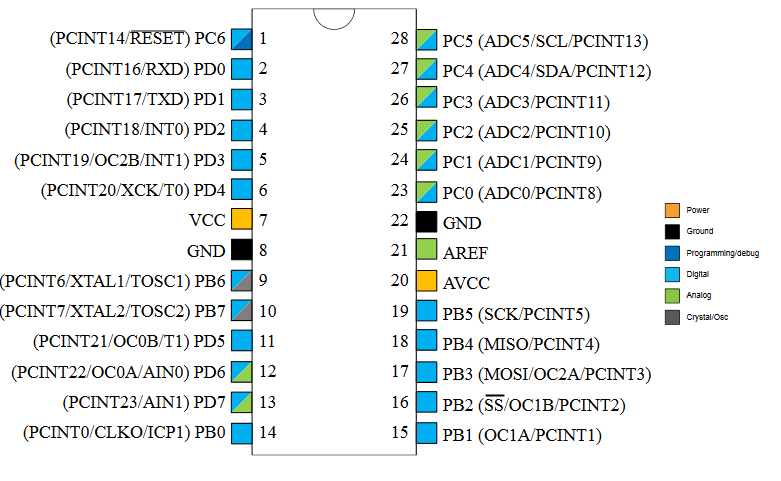
\includegraphics[width=0.9\textwidth]{Content/images/ATmega328P-pins}
	\caption{Pinout Diagram of the ATmega328P Micro Controller}
	\label{fig-atmega328p-pinout}
\end{figure}

\begin{figure}[p]
	\centering
	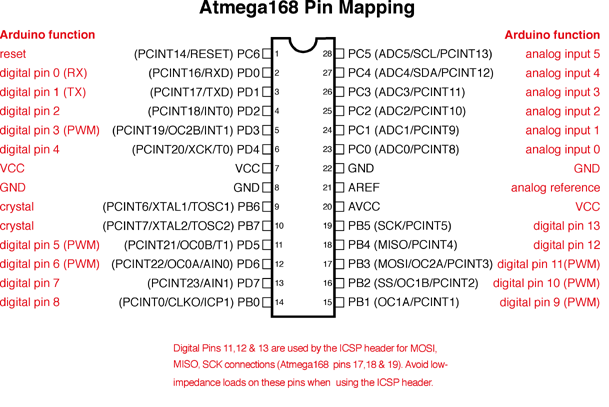
\includegraphics[width=0.9\textwidth]{Content/images/ArduinoUno-pins}
	\caption{Pinout Diagram of the ATmega328P showing Arduino Pin Use}
	\label{fig-arduino-uno-pinout}
\end{figure}

You may be wondering how, if the AVR pinout diagram shown in Figure~\ref{fig-atmega328p-pinout} doesn't have the Arduino's pin definitions, how the Arduino software is able to use the correct pins? This will be explained in section~\refname{avr-pinmodes} on page~\pageref{avr-pinmodes}.

\section{AVR Pinmodes}\label{avr-pinmodes}

You are most probably familiar with the \indexasis{Arduino}'s \inline{pinMode()} function, which allows you to define whether a pin is to be configured as input, output or input with pullup. You will not be surprised to find out that the AVR has a similar feature, but this one can do many pins at once.

However, as mentioned above, you may be wondering how the  \indexasis{Arduino} software gets from the \indexasis{Arduino} pin numbering format to those used on the actual AVR hardware? The process  as followed by \inline{pinMode()}, is as follows:

\begin{itemize}
	\item Convert the pin number to a \emph{bit mask} by calling \inline{digitalPinToBitMask()}.
	\item Convert the pin number to a port as well, by calling \inline{digitalPinToPort()}. If the port is invalid, do nothing and exit.
	\item Convert the (valid) port to a mode register by calling \inline{portModeRegister()}.
	\item Convert the (valid) port to a port output register by calling \inline{portOutputRegister()}.
	\item Preserve the current status register for the micro controller. Amongst other details, this will record the current state of the interrupts - whether or not they are currently enabled\footnote{See the data sheet for details of what the Status Register contains.}.
	\item Turn off any interrupts, even if already off. See \href{http://code.google.com/p/arduino/issues/detail?id=146}{This issue} for details of why this has to be done.
	\item Set the pin according to the desired mode - INPUT, INPUT\_PULLUP or OUTPUT.
	\item Restore the status register. This will also re-enable the interrupts, if they were enabled earlier.
\end{itemize}

That's an awful lot of work just to set a pin as OUTPUT, for example.

The functions \inline{digitalPinToBitMask()}, \inline{digitalPinToPort()}, \inline{portModeRegister()} and \inline{portOutputRegister()} are defined in the file:

\fbox{\inline{hardware/avr/cores/arduino/Arduino.h}}

which is located underneath wherever your \indexasis{Arduino} software is installed. If you ()only) have \indexasis{PlatformIO} installed, then the definitions are in:

\fbox{\inline{/home/norman/.platformio/packages/framework-arduinoavr/cores/arduino/Arduino.h}}

So, how does all of the above get us from the pin number 13, for pin D13, for example, to PB5? Well, the next section explains Ports and Pins, but briefly, calling \inline{pinMode(13, OUTPUT)} does all of the following:

\begin{itemize}
	\item \inline{digitalPinToBitMask(13)} returns a binary value of 0010 000, which is an 8 bit value, with bit 5 set to 1 and all other bits set to 0.
	\item \inline{digitalPinToPort(13)} returns the value 2, which is defined as a constant named ``PB''.
	\item \inline{portModeRegister(PB)} returns a pointer, this is C code remember, to the ``DDRB'' register. More on this in the following section.
	\item \inline{portOutputRegister(PB)} returns a pointer to ``PORTB''. More below on this too.
	\item Saves the status register.
	\item Turns off interrupts.
	\item Binary ORs the required bit of the ``DDRB'' register, bit 5 as above, with a 1, to set the pin to an output.
	\item Restores the status register (and interrupt state).
\end{itemize}

As I said, that's a lot of work, and a lot of code. In addition, there are a number of data tables written to the flash memory, where your program lives, to enable the above function calls to be facilitated. These tables take up $(3 * 10) + (3 * 20)$ or 90 bytes of potentially valuable program space.

That's for the \indexasis{Arduino}. For plain AVR C code, we set D13 (aka PortB, Pin 5) as follows:

\begin{lstlisting}[numbers={none}]
	DDRB |= (1 << 5);
\end{lstlisting}

Which is a lot less work, a lot fewer bytes overall and no tables are required. However, \emph{we}, the programmer, do have to remember the pin numbers etc.

The following section goes into greater detail about Pins and Ports.

\section{AVR Ports and Pins}\label{avr-ports-and-pins}

\subsection{Ports}\label{avr-ports}

The \indexasis{ATmega328P} has three separate ports named B, C and D. Other devices in the AVR family have additional ports, but we are restricted to the three already mentions.

The ports are named, simply enough, ``PORTB'', ``PORTC'' and ``PORTD''. Normally, each port will control up to 8 individual GPIO  pins, but on an Arduino, not all ports have the full set on pins.

A port, internally to the AVR, is simply an 8 bit register/memory address, connected via some complicated electronics, to the physical pins on the outside of the chip.

As far as we AVR and Arduino programmers, are concerned, we have the following ports (and therefore pins) available:

\begin{itemize}
	\item PORTB bits 0 to 5 = PB0 to PB5 = Arduino pins D8 to D13.
	\item PORTB bits 6 and 7 = PB6 and PB7. On the Arduino, these are used for the 16Mhz crystal and are not available as GPIO pins. Home brew setups can, if required, run off the micro controller's internal clock, and will be able to use these two pins.
	\item PORTC bits 0 to 5 = PC0 to PC5 = Arduino analogue pins A0 to A5.
	\item PORTC bit 6 = PC6 = the reset pin and, while it \emph{can} be fused as a GPIO pin, it is not usually configured in this manner. Doing so also disables the ability to reprogram the chip - unless you have a high voltage programmer. Best avoided!
	\item PORTD bits 0 to 7 = PD0 to PD7 = Arduino pins D0 to D7.
\end{itemize}

\subsubsection{Writing to an Output Port}\label{avr-ports-output-writing}
Writing a binary 1, to a bit in PORTx\footnote{The `x' refers to `B', `C' or `D'.} will set the connected GPIO pin high, if the pin is configured as an output of course. If it is configured as in input, writing a 1 will actually enable the input pullup resistor for  that pin.

\begin{lstlisting}[language=C,numbers={none}]
	// I want the  LEDs on PB5 to switch on, everything else off.
	PORTB = (1 << PB5);
}
\end{lstlisting}


\subsection{Pins}\label{avr-pins}

As mentioned above, each port in an AVR micro controller controls up to 8 GPIO pins. 

These GPIO pins can be configured as ``INPUT'', ``INPUT with PULLUP'' or ``OUTPUT''. 

In order to do this, there's a special register named the Data Direction Register, or ``DDR'' for each port. PORTA has DDRA, PORTB has DDRB and so on.

\subsubsection{Output Pins}\label{avr-pins-output}
In order to configure the pin PB5 (aka \indexasis{Arduino} D13) as an output, we set bit 5 to a 1. To configure as an input, we reset bit 5 of DDRB to a zero. You have seen the use of DDRB previously, in listing~\ref{lst-avrblink.c} where we did the following:

\begin{lstlisting}[language=C,numbers={none}]
	DDRB = (1 << PB5);
\end{lstlisting}

We could have also done the same thing as follows:

\begin{lstlisting}[language=C,numbers={none}]
	DDRB = (1 << DDB5);
\end{lstlisting}

or even:

\begin{lstlisting}[language=C,numbers={none}]
	DDRB = (1 << PORTB5);
\end{lstlisting}

This is because when we compile code for an \indexasis{ATmega328P}, there are certain values defined for us, and all of the above are defined as 5. They have different uses, but most AVR code that I've seen, uses the first version above. So I'll (probably) stick with that too. Feel free to use whatever version you are most comfortable with.

\begin{note}
	In general, if you want to set a bit in a register, or whatever, you can also use the \inline{\_BV} macro. This causes the \emph{compiler} to convert something like \inline{\_BV(5)} into \inline{(1 << 5)} but it is done at compile time so has no overhead at runtime.
	
	This means that there's another version of the code above to set bit 5 in DDRB, and that is:
	
	\begin{lstlisting}[language=C,numbers={none}]
		DDRB = _BV{5};	\end{lstlisting}	
\end{note}	

Of course, every version of the above is slightly incorrect. We do set bit 5 as desired, but we also reset all the other bits. This might affect your device especially as it may have already set some other bits to indicate output pins.

What we should have done is to binary ``OR'' the required pin values into the existing value in the DDR register, as follows:

\begin{lstlisting}[language=C,numbers={none}]
	DDRB |= (1 << PB5);
\end{lstlisting}

This will now \emph{only} affect bit 5, all the other bits remain unchanged.

We can set multiple pins as output, in the same command, as follows:

\begin{lstlisting}[language=C,numbers={none}]
	DDRB |= (1 << PB5)  | (1 << PB3);
\end{lstlisting}

Which will set pins PB3 and PB5 as outputs without affecting  the other pins.

\subsubsection{Input Pins}\label{avr-pins-input}

So far, we have seen how to set pins as output, equivalent to the \indexasis{Arduino}'s \inline{pinMode(pin, OUTPUT)} command. How then do we set a pin as input?

When the AVR is powered on, or reset, then the default setting for all pins is as input. However, it's best to be explicit. You could do this to set all the pins on PORTB to input mode:

\begin{lstlisting}[language=C,numbers={none}]
	DDRB = 0;
\end{lstlisting}

You could, but again, you are possibly reconverting some pins that have been set as outputs, elsewhere in your code. (Ask me how I know!) The best way is simply to binary ``AND'' a zero into the desired pin position, as follows:

\begin{lstlisting}[language=C,numbers={none}]
	DDRB &= ~(1 << PB5);
\end{lstlisting}

This creates a value with bit 5 set to a 1, and all other bits reset to zero, then flips it around so that all bits are set to 1 except bit 5. This is then ANDed with the current value in DDRB which has the effect of resetting bit 5 of DDRB to a zero, without affected any other bit.

As above, we can set multiple pins to be inputs quite simply:

\begin{lstlisting}[language=C,numbers={none}]
	DDRB &= ~((1 << PB5) | (1 << PB3));
\end{lstlisting}

This will set pins PB3 and PB5 as inputs without affecting other pins.

Ok, I hear you ask, we have output and input using a single bit per pin, so how do we get INPUT\_PULLUP like the \indexasis{Arduino}?

It was mentioned in passing above, but this is all you have to do:

\begin{itemize}
	\item Set the pin as an input in the normal manner.
	\item Write a 1 to the corresponding bit of the pin's PORTx register.
\end{itemize}

So, to set PB3 to an input, with pullup enabled, all we have to do is this:

\begin{lstlisting}[language=C,numbers={none}]
	// Configure PB3 as an input pin first.
	DDRB &= ~(1 << PB3);
	
	// Enable the pullup resistor on PB3.
	PORTB |= (1 << PB3);
\end{lstlisting}


\subsubsection{Reading From an Input Port}\label{avr-ports-input-reading}

To read the value of the pins configured as input, you simply read the value from the PINx\footnote{The `x' refers to `B', `C' or `D'.} register, for example:

\begin{lstlisting}[language=C,numbers={none}]
	uint8_t inputPins = PINB;
	if (inputPins & (1 << PB5)) {
		// Do something if pin PB5 is high.
	}
\end{lstlisting}


If a particular input pin is connected to ground (0 Volts) then the corresponding bit in the PINx register will be a zero. If a pin is connected to a \emph{high} voltage, then it will show a 1 in the corresponding bit of the appropriate PINx register.

Input pins with pullup\footnote{% complicated footnote ahead!
	I don't know about you, but I find it strange that a switch, for example, that is closed, returns a logical zero to the micro controller, rather than a 1 - which to me makes a lot more logical sense. Still, pullups! I would rather configure the pin as an input, with no pullup, and use an external \emph{pulldown} resistor to ground myself. That way, an open switch gives a zero bit in the appropriate PINx register, while a closed switch gives a 1. Or is that just me? 
	
	Yes, I \emph{know} that would be an additional cost when lots of pulldown resistors were required, in a commercial product, but I'm not making commercial products, and I have a bucket of resistors to use up!%
} will, of course, show a 1 unless pulled to ground by some external circuitry.





%\input{Content/Clock} % Clocks & crystals etc
\chapter{Timers}\label{avr-timers}

\section{Introdcution}\label{avr-timers-introduction}

\chapter{Interrupts}\label{avr-interrupts}

\section{Introduction}\label{avr-interrupts-introduction}

\chapter{Sleep Modes}\label{avr-sleep-modes}

\section{Introduction}\label{avr-sleep-modes-introduction}

%\input{Content/GPIO} % Digital Inputs & Outputs.
%\input{Content/PWM} % Analogue Outputs.
%\input{Content/USART} % Serial Communications
%\input{Content/ADC}
%\input{Content/BOD} %Brown Out Detector
%\input{Content/WDT} %Watch Dog Timer
%\input{Content/AC} %Analogue Comparator
%\input{Content/SPI} %Serial Peripheral Interface
%\input{Content/PowerSleep} %Power and Sleep modes
%\input{Content/TWI} % Two Wire Interface aka I2C


\part{A Worked Example}\label{part-worked-example}


% All the backend stuff, appendices, indexes etc.
%\backmatter

%\part{Appendices}\label{part-appendices}
%\chapterimage{ChapterImage.jpg} % Chapter heading image
%\begin{appendix}

\chapter{How the AVRBook Evolved}
\label{appendix-a-how-it-was-done}%\hyperlabel{appendix-a-how-it-was-done}%

To Be Completed.

There's a lot of work goes into this you know! ;-)


\end{appendix}

%\chapter{Using an Arduino as an ISP Programmer}
\label{using-an-arduino-as-an-isp-programmer}

\section{Introduction}\label{arduino-isp-introduction}

